\section{Experimental Protocol}
\label{sec:protocol}

\subsection{CIFAR-10}
We use CIFAR-10 \cite{cifar}: 50{,}000 training and 10{,}000 test images of
$32\times32$ pixels in ten classes, with class 0 as the attack target. Poisoning
is dirty-label: a fraction of non-target training images receive the trigger and
their labels are set to the target. BadNets stamps a $4\times4$ checkerboard of
alternating 1/0 pixels on rows and columns 27--30 \cite{badnets}. Blend replaces
the image by
$0.8x+0.2\pi$, where $\pi$ is a fixed uniform pattern generated with seed 123
\cite{blendattack}. The poison rate is 5\% (2{,}500 samples) except in the
amplification study, which uses 10\% (5{,}000 samples) to give the detector more
signal.

We train CIFAR variants of ResNet-18 \cite{resnet} and VGG-16-BN \cite{vgg} for
12 epochs with SGD (Nesterov momentum 0.9, weight decay
$5\times10^{-4}$), a OneCycle schedule with maximum learning rate 0.1 (0.05 for
VGG), batch size 512, random crop to $28\times28$ with padding 4, horizontal
flip, and mixed precision \cite{onecycle,bn,pytorch}. Normalisation is applied
inside the model. Three seeds (0, 1, 2) vary poison placement, initialisation,
and data order; the train/test split is fixed. Each seed therefore yields its own
gold model, and success is always judged against that seed's gold accuracy
($88.59$, $88.65$, and $88.77\%$ for seeds 0--2 respectively). The total CIFAR
compute was approximately 23 GPU-hours on two T4 cards.

Attack success is measured on the non-target test images after stamping the
trigger, so a model that predicts the target class indiscriminately cannot score
well by accident. Clean accuracy is measured on the unmodified test set.

\subsection{RadioML Automatic Modulation Classification}
The cross-domain study uses RadioML 2016.10a \cite{radioml,radioml_jstsp}: eleven
modulation classes, SNR from $-20$ to $18$\,dB in 2\,dB steps, each sample a
$2\times128$ in-phase/quadrature window. Samples are normalised to unit energy.
The classifier is a three-block one-dimensional CNN (32, 64, and 128 channels,
batch normalisation, max pooling, global average pooling) trained for 12 epochs
with Adam at learning rate $10^{-3}$ and weight decay $10^{-4}$. The trigger is
a fixed burst that sets $I{=}0.9$ and $Q{=}{-}0.9$ on the last eight samples,
and 5\% of the non-target training windows are stamped and relabelled to BPSK.
The split is 80/20 and fixed across seeds; poison placement and initialisation
vary. Removal methods are fine-tuned for four epochs at learning rate $10^{-4}$.
Four methods (gold retrain, retain fine-tuning, recipe, and inoculation-only) are
run at recall 1.0, 0.75, and 0.5 with precision 1.0, plus a precision-0.7 cell at
recall 0.75. Attack success and clean accuracy are evaluated per SNR bin.

We emphasise one protocol detail because it changes how the results must be read.
At SNR below about $-12$\,dB the clean classifier is close to chance (9.1\% for
eleven balanced classes), and an ASR threshold of 5\% is then not a
meaningful test of a defence: even the oracle retrain sits above it. We therefore
report $\gstar$ for every SNR but mark the near-chance region and restrict
interpretation to SNR at or above $-6$\,dB, where clean accuracy is at least
48\%.

\subsection{What Is Frozen}
The four experiment drivers were frozen before the final runs and were not
edited afterwards. Each driver writes one CSV row per run, including the
requested and realised recall and precision, the forget-set size, clean
accuracy, ASR, wall-clock time, and free-text notes. All figures and tables in
this paper are generated from those rows by a single analysis script; no
number was transcribed by hand. Where a run produced a degenerate detector
output (no flags, or flags containing no true poison) the row is kept in the
records and excluded from the corresponding table with a note. The logs are keyed
by person, experiment, architecture, attack, poison rate, seed, requested recall
and precision, method, and detector, so any table can be reconstructed by
filtering the logs; the analysis script applies those filters and writes the
\LaTeX{} tables and the PDF figures directly. Fig.~\ref{fig:arch} traces the
chain from the frozen core to the compiled PDF; because the analysis is a
deterministic function of the CSVs, every table can be regenerated without
rerunning a model.

\begin{figure*}[t]
\centering
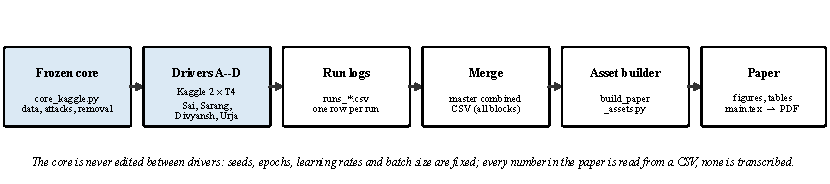
\includegraphics[width=\textwidth]{fig15_code_arch.pdf}
\caption{The artifact chain. Four frozen drivers write one CSV row per run, the
rows are merged into a master table, and the asset builder reads that table to
write the \LaTeX{} tables and PDF figures in this paper. No number is typed by
hand.}
\label{fig:arch}
\end{figure*}

\begin{table}[t]
\centering
\caption{Frozen experimental protocol. Every row of every table in this paper was produced under these settings; only the listed knobs vary between experiments.}
\label{tab:protocol}
\footnotesize
\begin{tabular}{@{}l >{\raggedright\arraybackslash}p{0.64\columnwidth}@{}}
\toprule
\textbf{Item} & \textbf{Setting} \\
\midrule
Dataset & CIFAR-10, 50k train / 10k test, 10 classes, target class 0 \\
Attacks & BadNets $4\times4$ checkerboard (rows/cols 27--30); Blend $0.8x+0.2\,\mathrm{pattern}$, seed 123 \\
Poison rate & 5\% (2{,}500 samples); 10\% in the amplification study \\
Architectures & ResNet-18, VGG-16-BN (CIFAR variants) \\
Optimiser & SGD, momentum 0.9 (Nesterov), weight decay $5\times10^{-4}$ \\
Schedule & OneCycleLR, max lr 0.1 (VGG 0.05), 12 epochs, batch 512 \\
Augmentation & random crop 32$\to$28 with padding 4, horizontal flip; normalisation inside the model \\
Seeds & 0, 1, 2 (identical splits; poison placement and init vary) \\
Detectors & Activation Clustering; Spectral Signatures (per-class, PCA/2-means resp.\ top singular vector) \\
Forget set & $\mathcal{F}(r,p)$: $N_p r$ true poison $+$ $N_p r(1-p)/p$ clean non-target false positives \\
Defence success & ASR $\leq5\%$ \emph{and} clean accuracy within 2 points of the gold retrain \\
Hardware & Kaggle 2$\times$T4 (16 GB each), mixed precision; $\approx$23 GPU-hours total \\
\bottomrule
\end{tabular}
\end{table}


\begin{table}[t]
\centering
\caption{Experiment blocks. E4 was planned and not executed; every other block is
reported in the section listed.}
\label{tab:blocks}
\footnotesize
\setlength{\tabcolsep}{3.5pt}
\begin{tabular}{@{}l >{\raggedright\arraybackslash}p{0.30\columnwidth} >{\raggedright\arraybackslash}p{0.34\columnwidth} c@{}}
\toprule
\textbf{Block} & \textbf{Question} & \textbf{What was run} & \textbf{Sec.} \\
\midrule
E1 & Does removal survive imperfect recall? & 10 $(r,p)$ cells $\times$ 5 methods $\times$ 3 seeds, ResNet-18/BadNets; inoculation-only baseline & VI \\
E2 & Is the cliff about residual poison? & 4 architecture--attack pairs $\times$ 5 residual fractions (0--100\%) & VI \\
E3 & Can calibration choose the threshold? & 20 SS thresholds with proxy removal; two full retrains & VIII \\
E4 & Does an adaptive attacker break the recipe? & planned, not executed & XII \\
E5 & Erasure or suppression? & 4 settings $\times$ relearning to 50 steps; MIA and KL probes & IX \\
E6 & Do real detector columns reproduce the cliff? & AC and SS at 1\%, 5\%, 10\% poison; deletion and recipe at realised operating points & VI \\
E7 & Does the cliff transfer? & VGG-16-BN/BadNets, VGG-16-BN/Blend, ResNet-18/Blend at $r{=}0.75,0.5$ & VII \\
E7b & Can the trigger be synthesised? & Neural-Cleanse synthesis on two attacks & VII \\
E8 & Is ascent removal real? & 4 ascent strengths $\times$ raw and BN-guarded & VIII \\
E9 & Does partial repair amplify detectability? & 10\% poison, 3 seeds $\times$ 2 repair strengths $+$ matched controls & VIII \\
SISA & How do efficiency-oriented baselines compare? & SISA-5 shards; fine-pruning at two thresholds & IX \\
RF & Does the cliff cross domains? & RadioML AMC, 4 methods $\times$ 3 recalls, 20 SNR bins, 3 seeds & X \\
\bottomrule
\end{tabular}
\end{table}


\subsection{Scope of the Evidence}
Table~\ref{tab:blocks} lists the experiment blocks, what each was run for, and
where it is reported. The CIFAR grid covers two architectures, two attacks,
three seeds, five removal families, and ten recall--precision cells; the
amplification study adds a third detector operating point at 10\% poison. The radio study covers one architecture,
one attack, three seeds, four methods, and twenty SNR bins. Two blocks that were
planned in the protocol were not executed: an adaptive-attacker study (E4) and a
full hyperparameter sweep for the baselines. We state this explicitly in
Section~\ref{sec:limits} rather than implying coverage we do not have. The claims
in this paper are correspondingly bounded: they concern post-training removal
under the stated attacks and budgets, not the impossibility of defence in
general.
